%% Copernicus Publications Manuscript Preparation Template for LaTeX Submissions
%% ---------------------------------
%% This template should be used for copernicus.cls
%% The class file and some style files are bundled in the Copernicus Latex Package, which can be downloaded from the different journal webpages.
%% For further assistance please contact Copernicus Publications at: production@copernicus.org
%% https://publications.copernicus.org/for_authors/manuscript_preparation.html

%% copernicus_rticles_template (flag for rticles template detection - do not remove!)

%% Please use the following documentclass and journal abbreviations for discussion papers and final revised papers.

%% 2-column papers and discussion papers
\documentclass[gc, manuscript]{copernicus}



%% Journal abbreviations (please use the same for preprints and final revised papers)

% Advances in Geosciences (adgeo)
% Advances in Radio Science (ars)
% Advances in Science and Research (asr)
% Advances in Statistical Climatology, Meteorology and Oceanography (ascmo)
% Annales Geophysicae (angeo)
% Archives Animal Breeding (aab)
% Atmospheric Chemistry and Physics (acp)
% Atmospheric Measurement Techniques (amt)
% Biogeosciences (bg)
% Climate of the Past (cp)
% DEUQUA Special Publications (deuquasp)
% Drinking Water Engineering and Science (dwes)
% Earth Surface Dynamics (esurf)
% Earth System Dynamics (esd)
% Earth System Science Data (essd)
% E&G Quaternary Science Journal (egqsj)
% EGUsphere (egusphere) | This is only for EGUsphere preprints submitted without relation to an EGU journal.
% European Journal of Mineralogy (ejm)
% Fossil Record (fr)
% Geochronology (gchron)
% Geographica Helvetica (gh)
% Geoscience Communication (gc)
% Geoscientific Instrumentation, Methods and Data Systems (gi)
% Geoscientific Model Development (gmd)
% History of Geo- and Space Sciences (hgss)
% Hydrology and Earth System Sciences (hess)
% Journal of Bone and Joint Infection (jbji)
% Journal of Micropalaeontology (jm)
% Journal of Sensors and Sensor Systems (jsss)
% Magnetic Resonance (mr)
% Mechanical Sciences (ms)
% Natural Hazards and Earth System Sciences (nhess)
% Nonlinear Processes in Geophysics (npg)
% Ocean Science (os)
% Polarforschung - Journal of the German Society for Polar Research (polf)
% Primate Biology (pb)
% Proceedings of the International Association of Hydrological Sciences (piahs)
% Safety of Nuclear Waste Disposal (sand)
% Scientific Drilling (sd)
% SOIL (soil)
% Solid Earth (se)
% The Cryosphere (tc)
% Weather and Climate Dynamics (wcd)
% Web Ecology (we)
% Wind Energy Science (wes)

% Pandoc citation processing

% The "Technical instructions for LaTex" by Copernicus require _not_ to insert any additional packages.
% 
% tightlist command for lists without linebreak
\providecommand{\tightlist}{%
  \setlength{\itemsep}{0pt}\setlength{\parskip}{0pt}}


%
\begin{document}


\title{New insights into the Weddell Sea ecosystem applying a network
approach}


\Author[1, *]{Tomás I.}{Marina}
\Author[1, *]{Leonardo A.}{Saravia}
\Author[2]{Susanne}{Kortsch}


\affil[1]{Centro Austral de Investigaciones Científicas (CADIC-CONICET),
Ushuaia, Argentina}
\affil[2]{University of Helsinki, Helsinki, Finland}
\affil[*]{These authors contributed equally to this work.}

\runningtitle{New insights into the Weddell Sea food web}

\runningauthor{Marina et al.}

\correspondence{Tomás I. Marina (tomasimarina@gmail.com) and Leonardo A.
Saravia (arysar@gmail.com)}


\received{}
\pubdiscuss{} %% only important for two-stage journals
\revised{}
\accepted{}
\published{}

%% These dates will be inserted by Copernicus Publications during the typesetting process.


\firstpage{1}

\maketitle


\begin{abstract}
The abstract goes here. It can also be on \emph{multiple lines}.
\end{abstract}




\introduction[Introduction]

The objective of this work was threefold: 1) estimate the strength for
each interaction in the Weddell Sea food web, 2) characterise species
considering weighted and unweighted properties, and 3) analyse the
species' role in the stability of the food web.

\section{Methodology}

\subsection{Study area}

The high Antarctic Weddell Sea shelf is situated between 74 and 78ºS
with a length of approximately 450 km (Figure 1). Water depth varies
from 200 to 500 m. Shallower areas are covered by continental ice, which
forms the coastline along the eastern and southern part of the Weddell
Sea. The shelf area contains a complex three-dimensional habitat with
large biomass, intermediate to high diversity in comparison to benthic
boreal communities and a spatially patchy distribution of organisms
\citep{Dayton1990, Teixido2002}.

\subsection{Weddell Sea food web dataset}

We obtained the dataset of the Weddell Sea food web from the GlobAL
daTabasE of traits and food Web Architecture (GATEWAy, version 1.0) of
the German Centre for Integrative Biodiversity Research (iDiv)
Halle-Jena-Leipzig \citep{Brose2018}. This open access database is a
list of predator-prey interactions that contains several highly-resolved
food webs, including biological data about the consumer and resource
species involved in each trophic interaction (i.e.~mean mass).
Furthermore, it incorporates information about the interaction itself,
such as the dimensionality (2 or 3 dimensions).

This marine food web compiles all the trophic data available for the
high Antarctic Weddell Sea collected since 1983, and is one of the most
highly-resolved marine food webs documented to date. It's noteworthy
that it is a summary network that ignores seasonal changes
\citep{Jacob2011}.

\subsection{Dataset analyses}

We analysed the food web of the Weddell Sea by: a) estimating the
strength of each interaction; b) studying the species properties in a
network framework; and c) comparing the stability of the food web after
performing species extinction in silico simulations.

\subsubsection{Interaction strength estimation and distribution}

To estimate the strength of each interaction in the food web we followed
the methodology proposed by \citet{Pawar2012}. The minimum data
requirements are: body mass of the consumer (predator) and resource
(prey), and the interaction dimensionality classified as 2 or 3
dimensions. GATEWAy v.1.0 does provide the mean mass for consumers and
resources (except for `detritus' and `sediment') and the dimensionality
for the majority of the interactions, though the latter is missing in
some cases (924 interactions). To complete such missing data, we used
information about movement type for consumer and resource included in
GATEWAy. Thus, we classified the interaction as 2D if both consumer and
resource move in 2D (e.g., both are sessile or walking) or if a consumer
moves in 3D and a resource in 2D (e.g., swimming consumer and
sessile/walking resource). The interaction was classified as 3D if both
consumer and resource move in 3D (e.g., both swimming) or if the
consumer moves in 2D and the resource in 3D (e.g., sessile/walking
consumer, swimming resource) \citep{Pawar2012}.

The main equation we used for estimating the interaction strength IS
was:

\begin{equation}
IS = \alpha x_R \frac{m_R}{m_C}
\end{equation}

where \vec{\alpha} is the search rate, \vec{x_R} is the resource
density, and \vec{m_R} and \vec{m_C} are the body mass for the resource
and the consumer, respectively \citep{Pawar2012}.

We obtained estimations for the resource density and the search rate
from the scaling relationships with the resource and the consumer mass,
respectively \citep{Pawar2012}. The coefficients of such relationships,
determined by ordinary least squares regression, vary with the
interaction dimensionality. On one hand, resource density scales with
resource mass as power-law with exponents \vec{p = -0.79 \pm 0.09} in 2D
and \vec{p = -0.86 \pm 0.06} in 3D. Since mean mass for resources
`phytodetritus' and `sediment' were not available in GATEWAy, we
considered the body mass of the smallest phytoplankton species
(`Fragilariopsis cylindrus') as a proxy. This is justified by the fact
that `phytodetritus' and `sediment' are mainly composed by dead or
senescent phytoplankton reaching the seabed (\citet{Wolanski2011}). On
the other hand, search rate scales with consumer mass as power-law with
exponents \vec{p = 0.68 \pm 0.12} in 2D and \vec{p = 1.05 \pm 0.08} in
3D.

Finally, we fit the interaction strength distribution of the food web
considering six candidate models (Exponential, Gamma, log-Normal,
Normal, Power-law and Uniform) using maximum likelihood
\citep{McCallum2008}, and selected the model performance by computing
the Akaike Information Criterion AIC \citep{Burnham2002}.

\subsubsection{Species properties}

In order to individually characterize the species of the food web, we
considered weighted and unweighted properties (Figure 2). The former is
based on the estimation of the interaction strength described in the
previous section. The latter is related to properties commonly used in
qualitative or topological (presence/absence of interaction) food web
studies \citep{Martinez1991, Dunne2002, Borrelli2014}.

As the weighted property we took into account the total mean interaction
strength, meaning the average strength of all species' interactions for
each species. On the other hand, we considered the following unweighted
properties: a) degree or the total number of trophic interactions,
summing up in- and out-coming interactions (role as predator and prey,
respectively); b) trophic level or the position in the food web relative
to primary producers/detritus; and c) trophic similarity or the trophic
overlap based on shared and unique resources and consumers. The
following are arguments to have selected the unweighted properties. The
degree has often been equated with importance to the structure and
functioning of a community, i.e.~perturbations to high-degree species
may therefore have larger effects on the food web than perturbations to
low-degree species \citetext{\citealp{Dunne2002a}; \citealp[references
in][]{Cirtwill2018a}}. The trophic level offers information about how
important a species is to its biotic community, i.e.~top predators and
primary producers are expected to have particularly large effects on the
rest of their communities through top-down and bottom-up control,
respectively \citep[references in][]{Cirtwill2018a}. The trophic
similarity measures one of the most important aspects of species'
niches, the trophic niche, and functional aspects of biodiversity
\citep{Martinez1991, Williams2000}.

Furthermore, we took into account the species' habitat, which describes
the physical position of a species within the ecosystem. Species were
categorized as: 1) benthic, if the species lives on the seafloor; 2)
pelagic, if the species lives close to the surface; 3) benthopelagic, if
it moves between and connects the mentioned environments; 4) demersal,
if it lives and feeds on or near the bottom of the sea; and 5)
land-based, if the consumer is not aquatic but feeds predominantly in
the marine realm. These data was taken from \citet{Jacob2011}.

With the aim of studying the relationship between the interaction
strength of the species (weighted property) and its unweighted
properties we performed linear regression analyses between the log(mean
interaction strength) and each of the mentioned unweighted properties.
We also explored such weighted property with species habitat.

Formulas used to obtain the above species properties are described in
Supplementary Material.

\subsubsection{Extinction simulations and stability}

Finally, we run extinction simulations and estimated its impact on the
stability of the food web. For this, we calculated a stability index
called Quasi-Sign Stability (QSS), which is the proportion of stable
networks using randomized Jacobians and keeping the predator-prey sign
structure fixed \citep{Allesina2008}. If this proportion is zero, then
one should take into account the real part of the maximum eigenvalue of
the Jacobian matrix, which is also a measure of stability
\citep{Grilli2016}.

With the aim of analysing the effect of each species on the food web's
stability we performed extinction simulations deleting one species at a
time, so the network size was reduced by one. After each species
extinction, we calculated the stability for the food web minus one
species (size = 489) and compared it with that of the whole network
(size = 490). We performed 1000 simulations for each species extinction
and obtained a mean QSS and maximum eigenvalue. At last we statistically
analysed such difference with an Anderson-Darling test considering a
p-value \textless{} 0.01 \citep{Scholz1987}. If the difference was
positive, then the stability of the food web was impacted positively
(higher stability) when that species become extinct, and viceversa.
Details for the stability calculations are described in Supplementary
Material.

Once we had the results for the impact on stability for each species
extinction, we plotted them considering weighted (interaction strength)
and unweighted properties, and species habitat. With this we aim to
characterize those species with a relatively high effect on the
stability of the food web.

All analyses were performed in R software, mainly using packages igraph
\citep{Csardi2005}, cheddar \citep{Hudson2013}, and multiweb
\citep{Saravia2019}. The source code and data are available at
https://github.com/EcoComplex/WeddellSea.

\section{Results}

\subsection{Interaction strength}

In this work we have estimated the interaction strength for the most
highly-resolved marine food web to date, which comprises 490 species and
16041 predator-prey interactions. The distribution of the interaction
strength best fit to a log-Normal model, meaning that there is a
prevalent skew towards weaker interactions (Figure 3, Table 1).

\subsection{Species properties}

Following the above results for the distribution of the interaction
strengths, we found that the species mean interaction strength was
different. We also found that such weighted property is related more or
less with unweighted properties (Figure 4A-D). In this regard,
interaction strength - trophic level showed a significant positive
linear regression: the higher the trophic level of the species, the
higher its mean interaction strength. We also found a significant but
less evident positive relationship with degree or the total number of
interactions. On the other hand, there was no significant relationship
with trophic similarity. Considering species habitat, the
``Benthopelagic'' and ``Pelagic'' categories presented the two species
with the highest mean interaction strength (Orcinus orca and
Mesonychoteuthis hamiltoni, respectively), though ``Demersal'' and
``Land-based'' habitats concentrated the majority of the species with
relatively higher interaction strength. Species inhabiting the benthic
realm showed the lowest mean interaction strength (Figure 4D).

\subsection{Extinction simulations and stability}

It's important to note that since the proportion of Jacobians that are
locally stable or QSS was zero for the Weddell Sea food web, we
considered the mean maximum eigenvalue as the stability index. When
performing the extinction simulations, our results showed that the
majority of the species had no significant impact on the stability of
the food web when extinct (Figure 5). This is shown in Figure 5, where
most of the points lie around the zero value of the `Stability
difference' y axis, meaning that the stability for the food web minus a
given species is similar (not significant) to the stability for the
whole network. However, there were few species that when become extinct
altered significantly the stability of the food web. Most of such
species generated positive significant differences in the stability of
the food web, which mean that they increased the network's stability
when deleted. There were two exceptions, Pagetopsis macropterus
(demersal fish) and Maxilliphimedia longipes (benthopelagic amphipod),
that when deleted decreased the stability. Overall, 15 out of 490
species (3.06\%) gave rise to significant changes in the food web's
stability (Table 2).

After exploring the stability difference against the species properties
(Figure 5), we found that those species that generated a significant
impact on the stability of the food web were characterized by: 1) high
mean interaction strength; 2) mid to high trophic levels (TL
\textgreater{} 3.2); 3) relatively high number of interactions (Degree
\textgreater{} 25); and 4) mid to low trophic similarity (TS \textless{}
0.16). Habitat wise, species with a significant impact on the stability
were present in all habitats, except for the benthic realm. Table 2
shows these results for such species.

\section{Discussion}

Using the highest-resolved marine polar food web up to date, we show
that 1) the distribution of the interaction strength at the food web
level is asymmetric, where weak interactions are prevalent; that 2)
there is a positive relationship between species mean interaction
strength and two unweighted properties, trophic level and degree; and
that 3) only few species are key in terms of food web stability,
presenting particular weighted and unweighted properties. It's also
noteworthy, that our study is the first of its type to consider the
dimensionality of the interaction (2 or 3 dimensions) to estimate
predator-prey relationships within a food web framework. After analysing
more than 2900 predator-prey interactions from several ecosystems,
\citet{Pawar2012} concluded that interaction dimensionality is a
critical factor driving consumer-resource dynamics, which will lead to
better predictions of food web and ecosystem functioning. This arises as
crucial to better understand how a complex system such as the Weddell
Sea might respond to environmental change, which is an ongoing issue in
that region of the Antarctic \citep[ and references herein]{Gutt2022}.

Our results regarding the distribution of the interaction strengths are
consistent with prior theoretical and empirical studies
\citep[e.g.][]{McCann1998, Neutel2002, Emmerson2004, Wootton2005}.
Within a system of a given complexity, commonly only a few strong
species interactions are present with most interactions being weak.
Historically, after \citet{May1972} installed the debate
complexity-stability, the results about the distribution of the
interaction strength has been interpreted as an explanation for the
persistence of complex food webs in nature
\citep{Bascompte2005, Allesina2015, Nilsson2016}. Here we showed that
this pattern is also prevalent in one of the most complex empirical
marine food webs that was studied so far, with 490 species and 16041
predator-prey interactions.

Our approach to study species properties follows \citet{Kortsch2021}
recommendation that suggests to employ a range of descriptors from both
unweighted and weighted food web in order to characterise the dynamic
and multifaceted nature of structural and functional ecosystem changes.
We went a step forward and analysed the relationship between weighted
and unweighted descriptors. In this regard, our results show a positive
relationship between interaction strength (weighted) and trophic level
(unweighted), and between interaction strength and degree (total number
of interactions). The former relationship might contradict those studies
that suggest that mid-trophic level species are involved in the major
pathways of energy flow in high-latitude marine ecosystems
\citep{Pinkerton2014, Murphy2016, McCormack2020, Riccialdelli2020}. This
could be explained by the lack of species biomass data in our
interaction strength estimations; the methodology we applied here
\citep{Pawar2012} allows to include empirical data for the density of
the resource, though not for all food web species. Unfortunately, the
lack of individual data for the entire Weddell Sea food web hampers any
alternative approach. On the other hand, the positive relationship
between interaction strength and degree reinforces the importance of
species with many interactions: species with high degree (hubs) have a
large impact on overall food web structure and functioning
\citep{Dunne2002a, Kortsch2015}. In the Weddell Sea, species with high
degree also tend to have high mean interaction strengths. This
information on the quantity and quality of interactions and its
relationship enables a robust assessment of the species' role in the
stability of the food web \citep{Cirtwill2018a}.

Our results show that only few species are key in terms of stability in
the Weddell Sea food web. This is in concordance with studies of complex
empirical food webs in marine ecosystems in the Arctic and other
locations in Antarctica \citep{Kortsch2015, Marina2018, Rodriguez2022}.
In the present work we identify that such key species present particular
weighted and unweighted properties: 1) high mean interaction strength;
2) mid to high trophic level; 3) relatively high number of interactions;
and 4) mid to low trophic similarity. The first attempt to gain insight
into the role of species in the Weddell Sea applying a complex approach
was that of \citet{Jacob2011}. These authors used information on body
size, predatory and feeding type, and environment (habitat) to study
species' roles. After performing sequential extinction simulations,
\citet{Jacob2011} found that larger bodied species can be lost without
causing a direct collapse of the network topology. A major caveat of
this finding, already recognized by the authors, is that population
dynamics were ignored and therefore no top-down extinctions, or other
indirect effects, could occur. In our study we did consider such effects
by including information on the species interaction strength, which is
of paramount importance when analysing the response of perturbations in
ecological communities \citep{McCann1998, Montoya2009, Novak2011}. Thus,
our study suggests that species with high mean interaction strength and
high trophic level need to be considered with particular attention when
trying to predict the effects of perturbations on the Weddell Sea
ecosystem. Furthermore, this arises as a greater issue since we have
identified that these species present a mid to low trophic similarity,
meaning that few other species of the food web can occupy the same
trophic role. In this sense, \citet{Murphy2016}'s review emphasized that
polar pelagic ecosystems are particularly sensitive to change due to a
low functional redundancy at key trophic levels. It's important to note
that we provide a broader analysis in this regard because we have
included species from all habitats (pelagic, benthic, land-based).

\clearpage
\conclusions[Conclusions]

Our study goes beyond the current understanding of how species influence
ecosystem structure and stability in the Weddell Sea in particular and
in most polar regions in general \citep{Murphy2016, McCormack2021}. In
the same analysis we have integrated information about weighted
(interaction strength) and unweighted species properties, enabling a
more complete assessment of the food web structure and function, likely
highlighting the ecological processes at play in the Weddell Sea
ecosystem.

We consider that the information provided in this study is important for
the development of effective policies and management strategies,
particularly given the ongoing initiative to implement a Marine
Protected Area (MPA) in the Weddell Sea \citep{Teschke2021}.

\clearpage

\begin{figure}
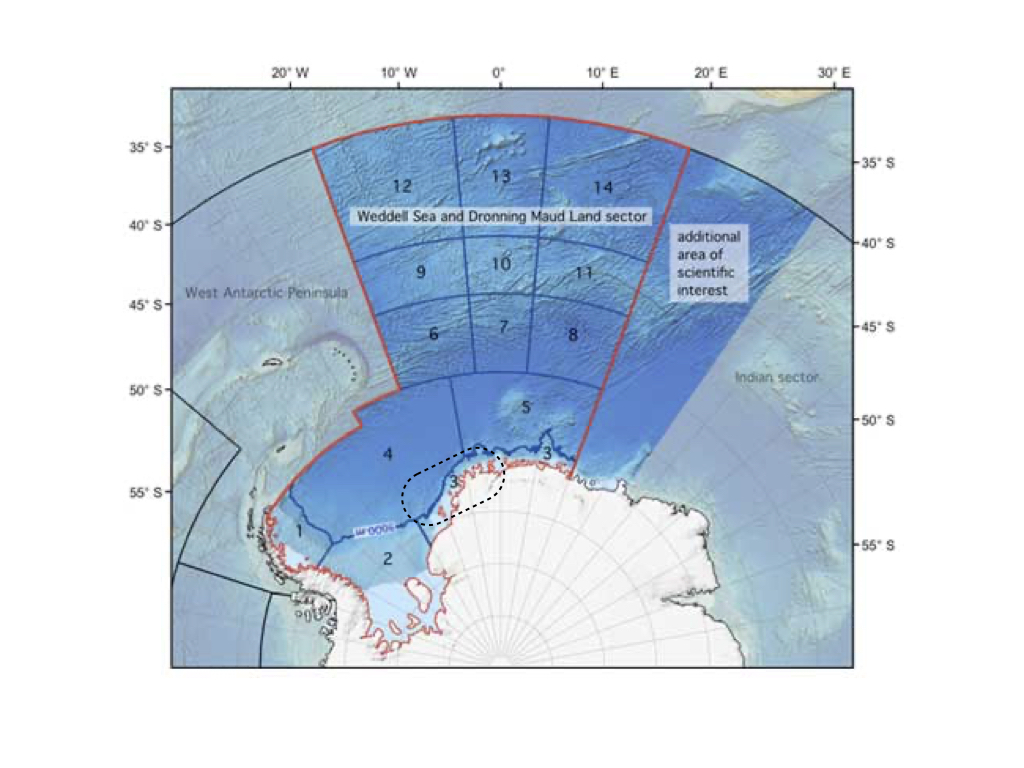
\includegraphics[width=12cm]{Fig.1_StudyMap} \caption{Map of the Weddell Sea and Dronning Maud Land sector highlighting the high Antarctic shelf as a dashed-line contour. Modified from www.soos.aq.}\label{fig:unnamed-chunk-1}
\end{figure}

\clearpage

\begin{figure}
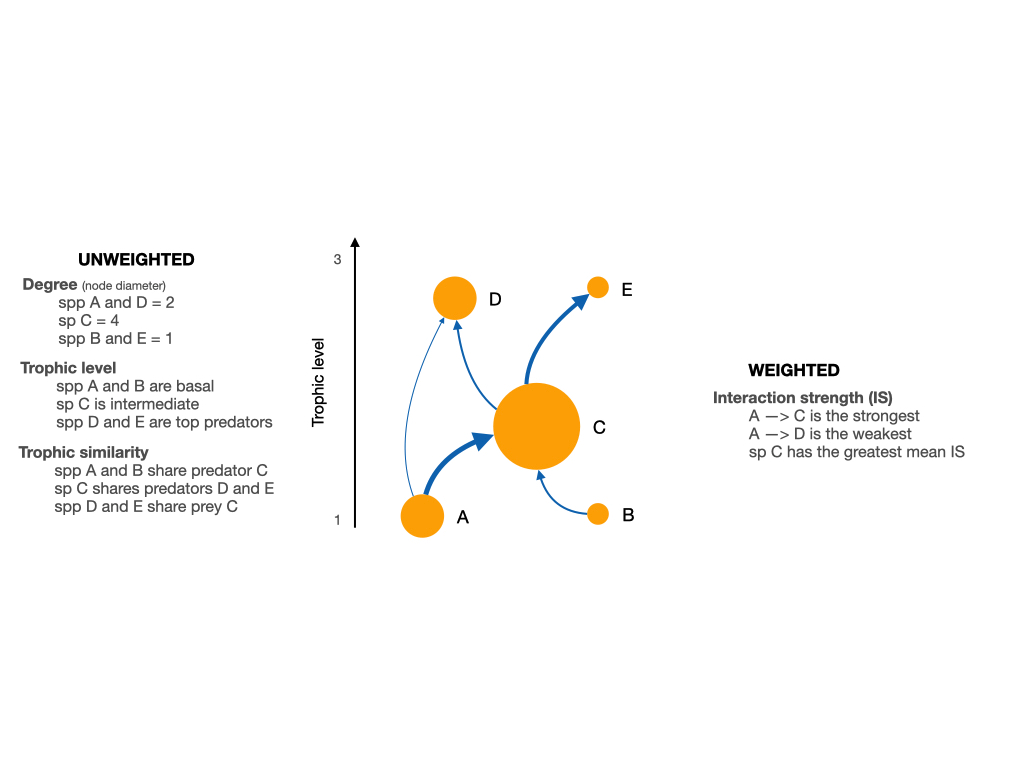
\includegraphics[width=12cm]{Fig.2_ToyFoodWeb} \caption{Scheme of a network showing the weighted and unweighted properties we used to characterize the species of the Weddell Sea food web.}\label{fig:unnamed-chunk-2}
\end{figure}

\clearpage

\begin{figure}
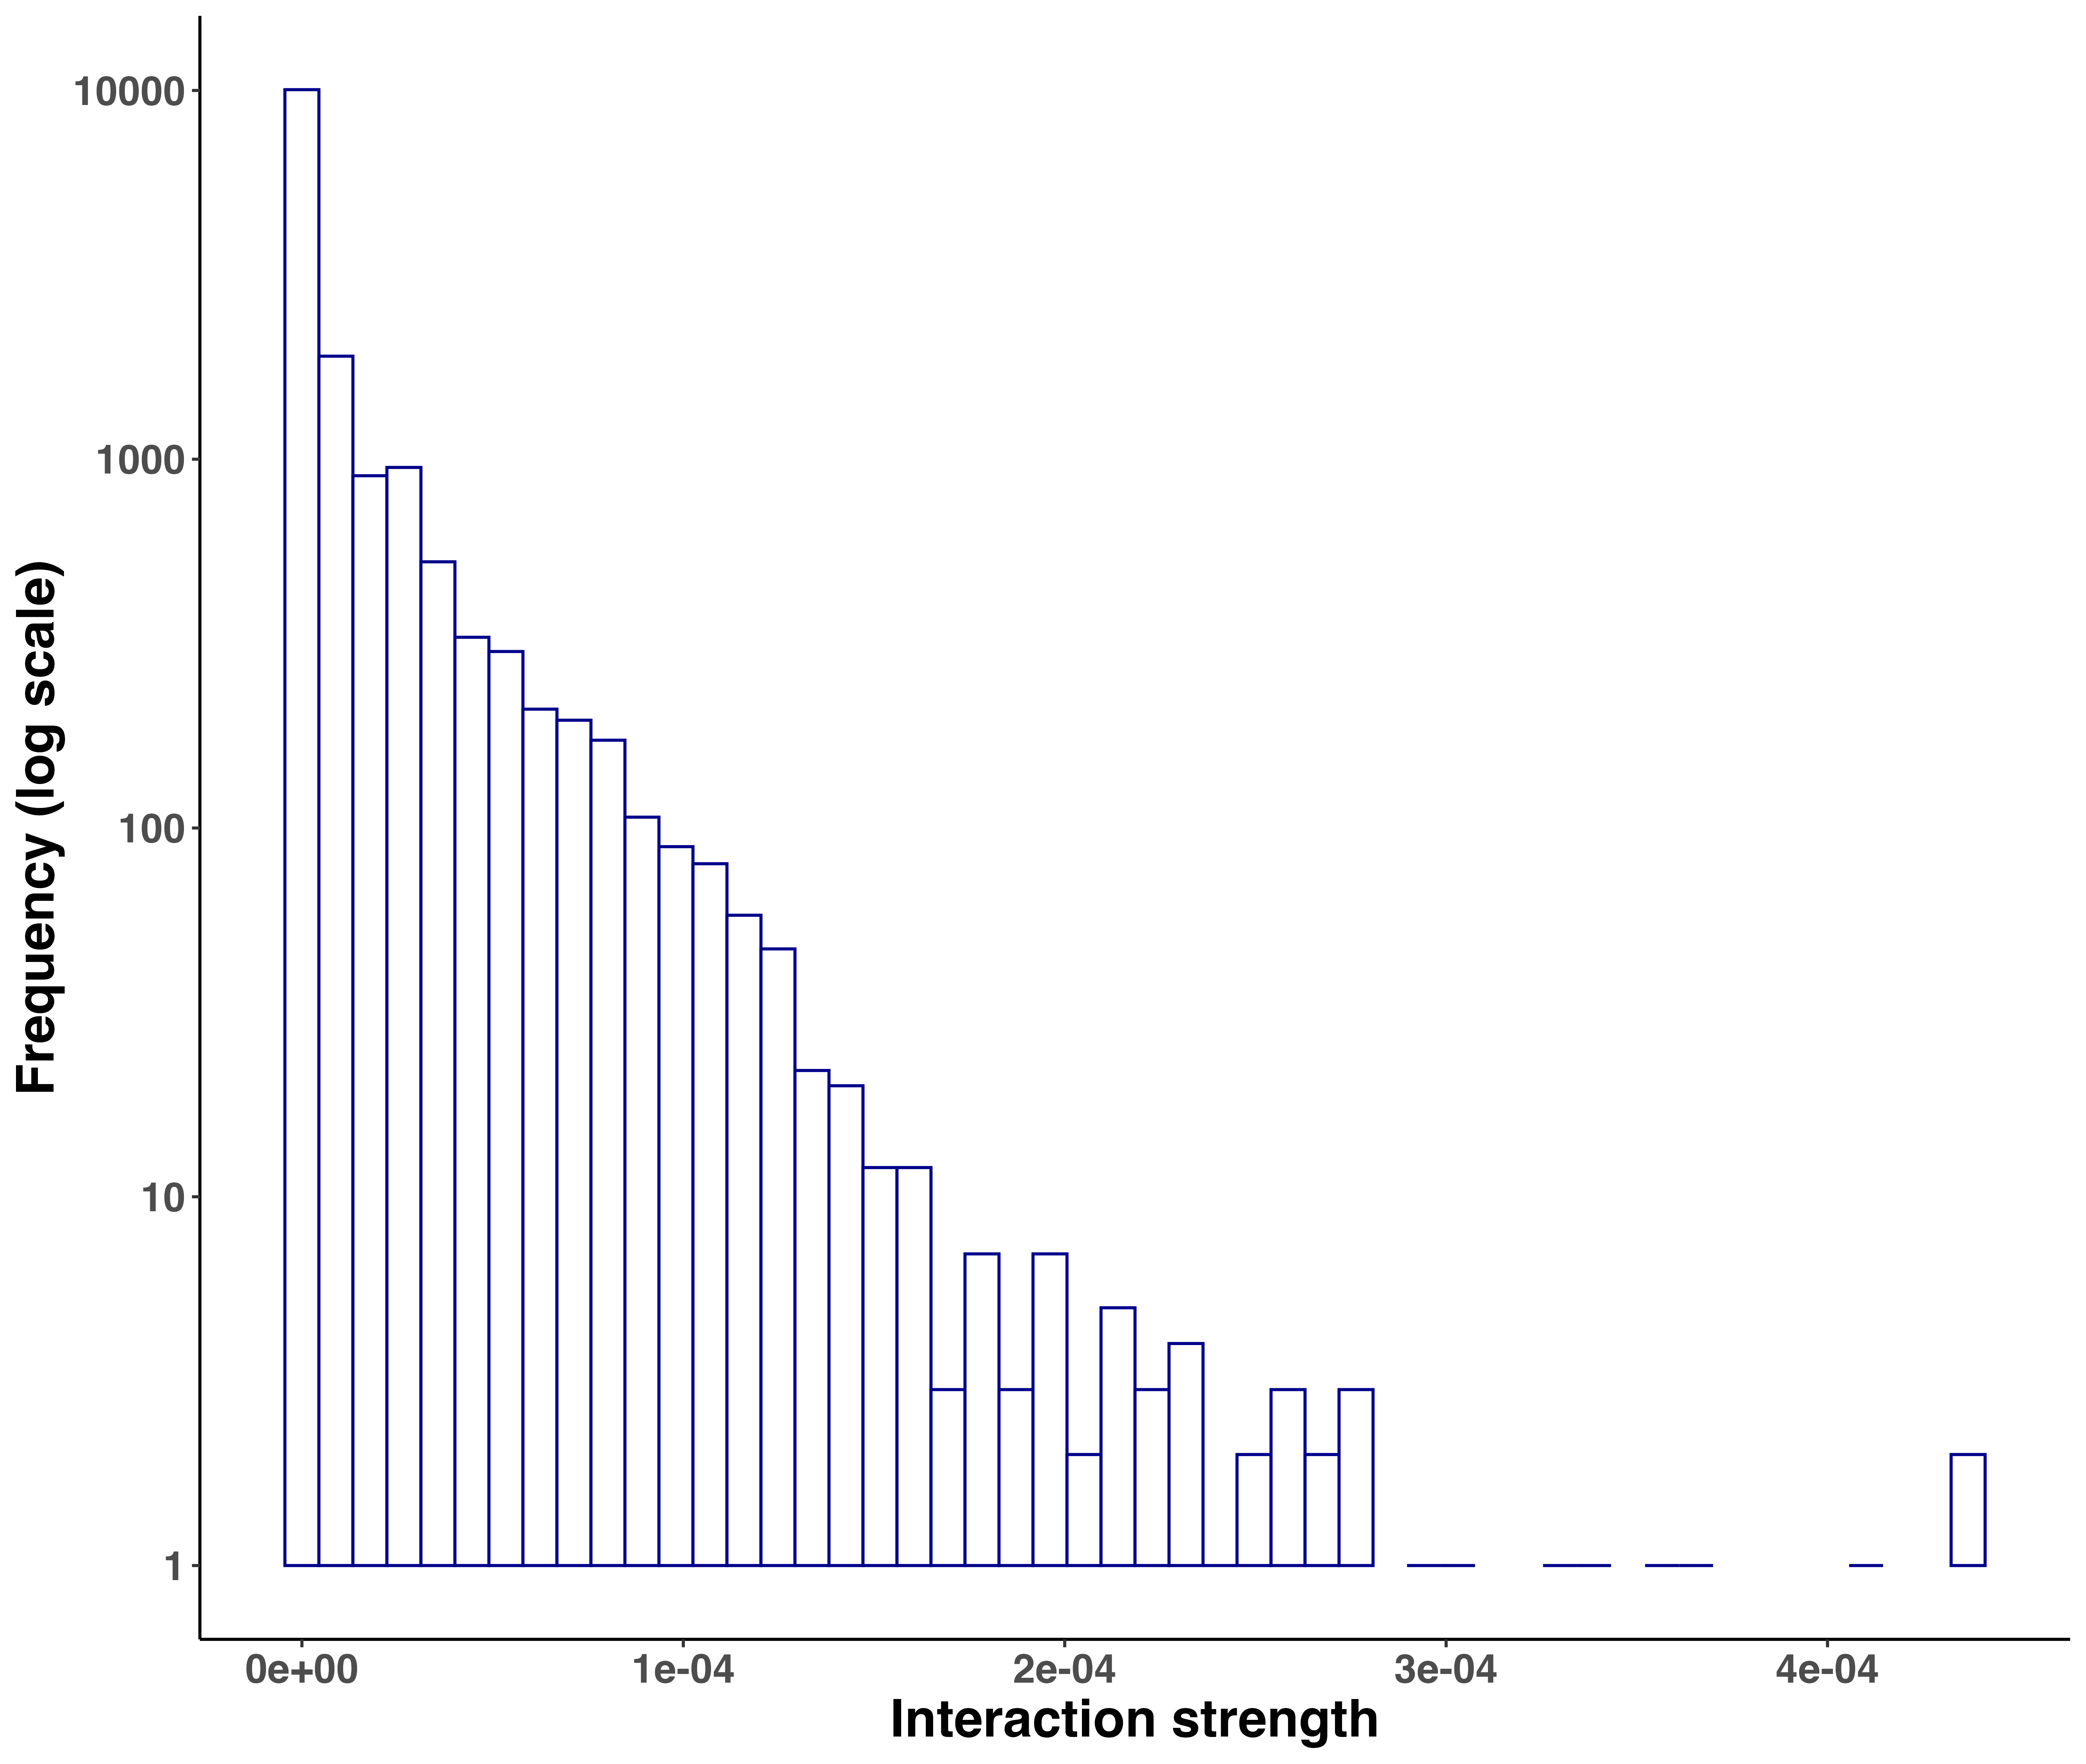
\includegraphics[width=12cm]{Fig3_IntDist} \caption{Frequency distribution of interaction strengths for the Weddell Sea food web. Total number of interactions = 16041.}\label{fig:unnamed-chunk-3}
\end{figure}

\clearpage

\begin{figure}
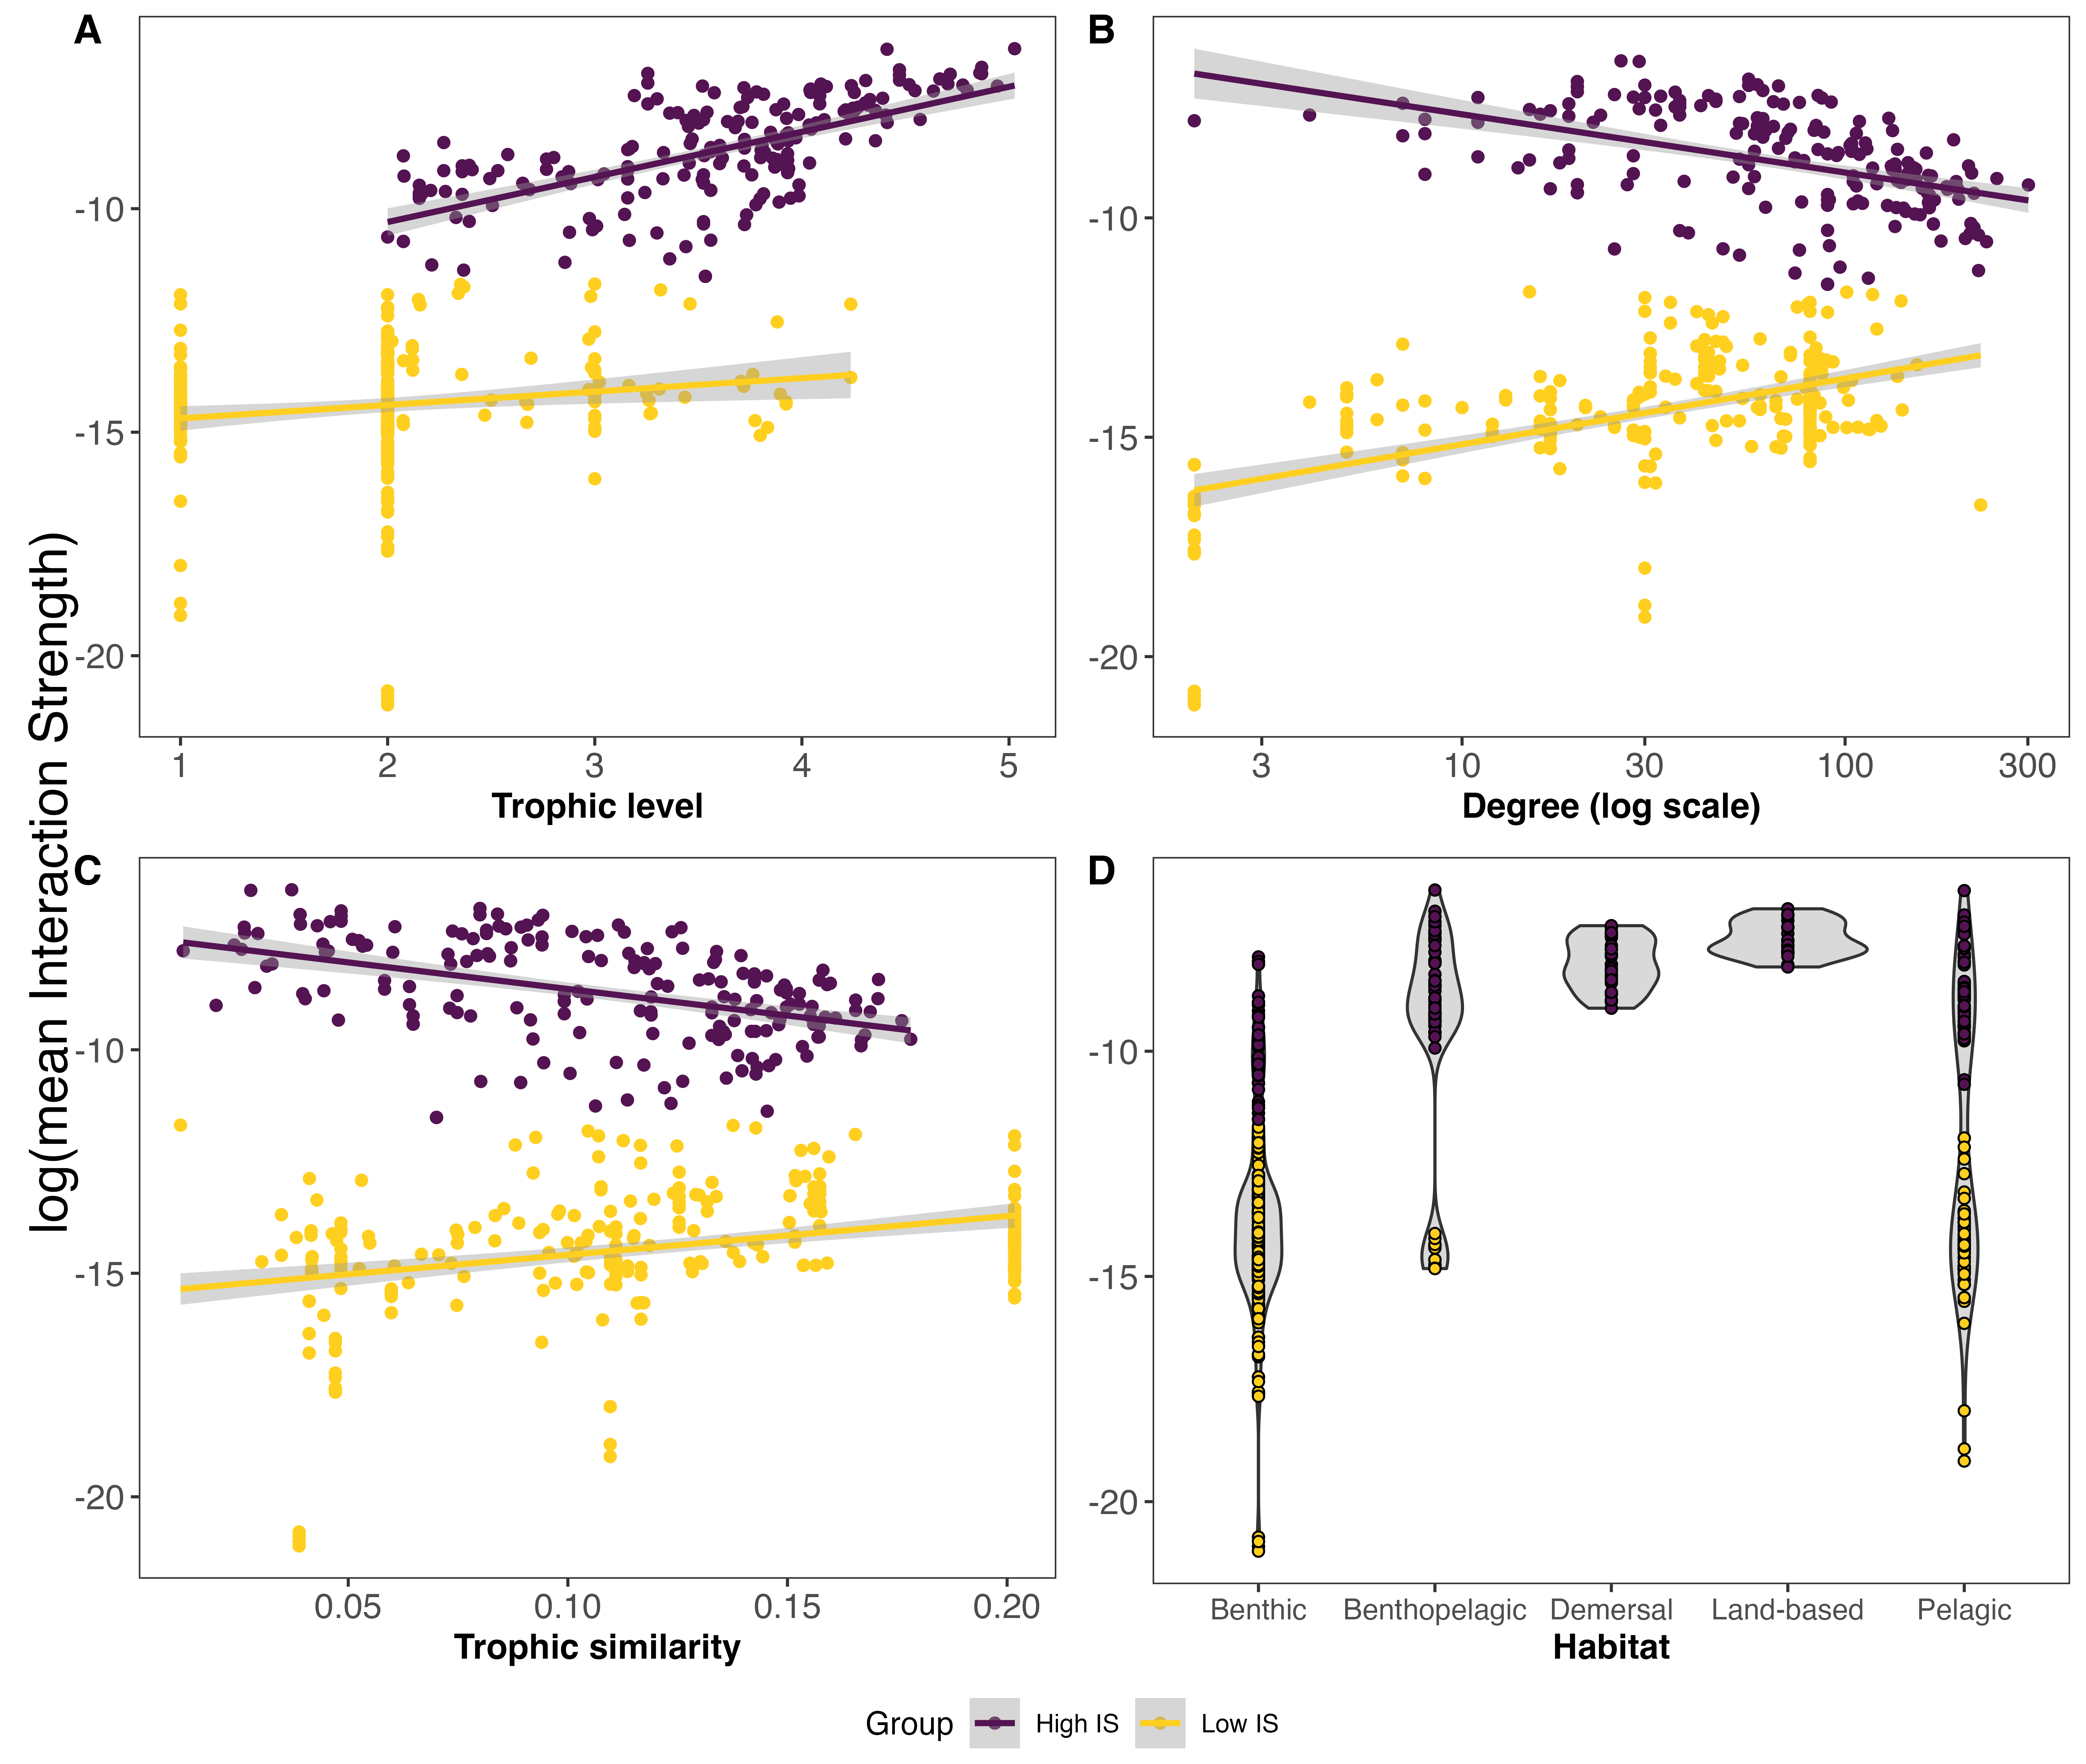
\includegraphics[width=12cm]{Fig4_LinReg} \caption{Relationships between weighted (mean Interaction Strength) and unweighted properties including habitat. Linear regressions are shown between log(mean interaction strength) and trophic level (A), degree (B) and trophic similarity (C). Linear regressions for trophic level ($y = 1.12x - 15.29, R^2 = 0.43, p-value < 2e-16$), degree ($y = 0.006x - 12.77, R^2 = 0.03, p-value = 4.06e-5$) and trophic similarity ($y = -1.46x - 12.18, R^2 = -0.0004, p-value = 0.36$).}\label{fig:unnamed-chunk-4}
\end{figure}

\clearpage

\begin{figure}
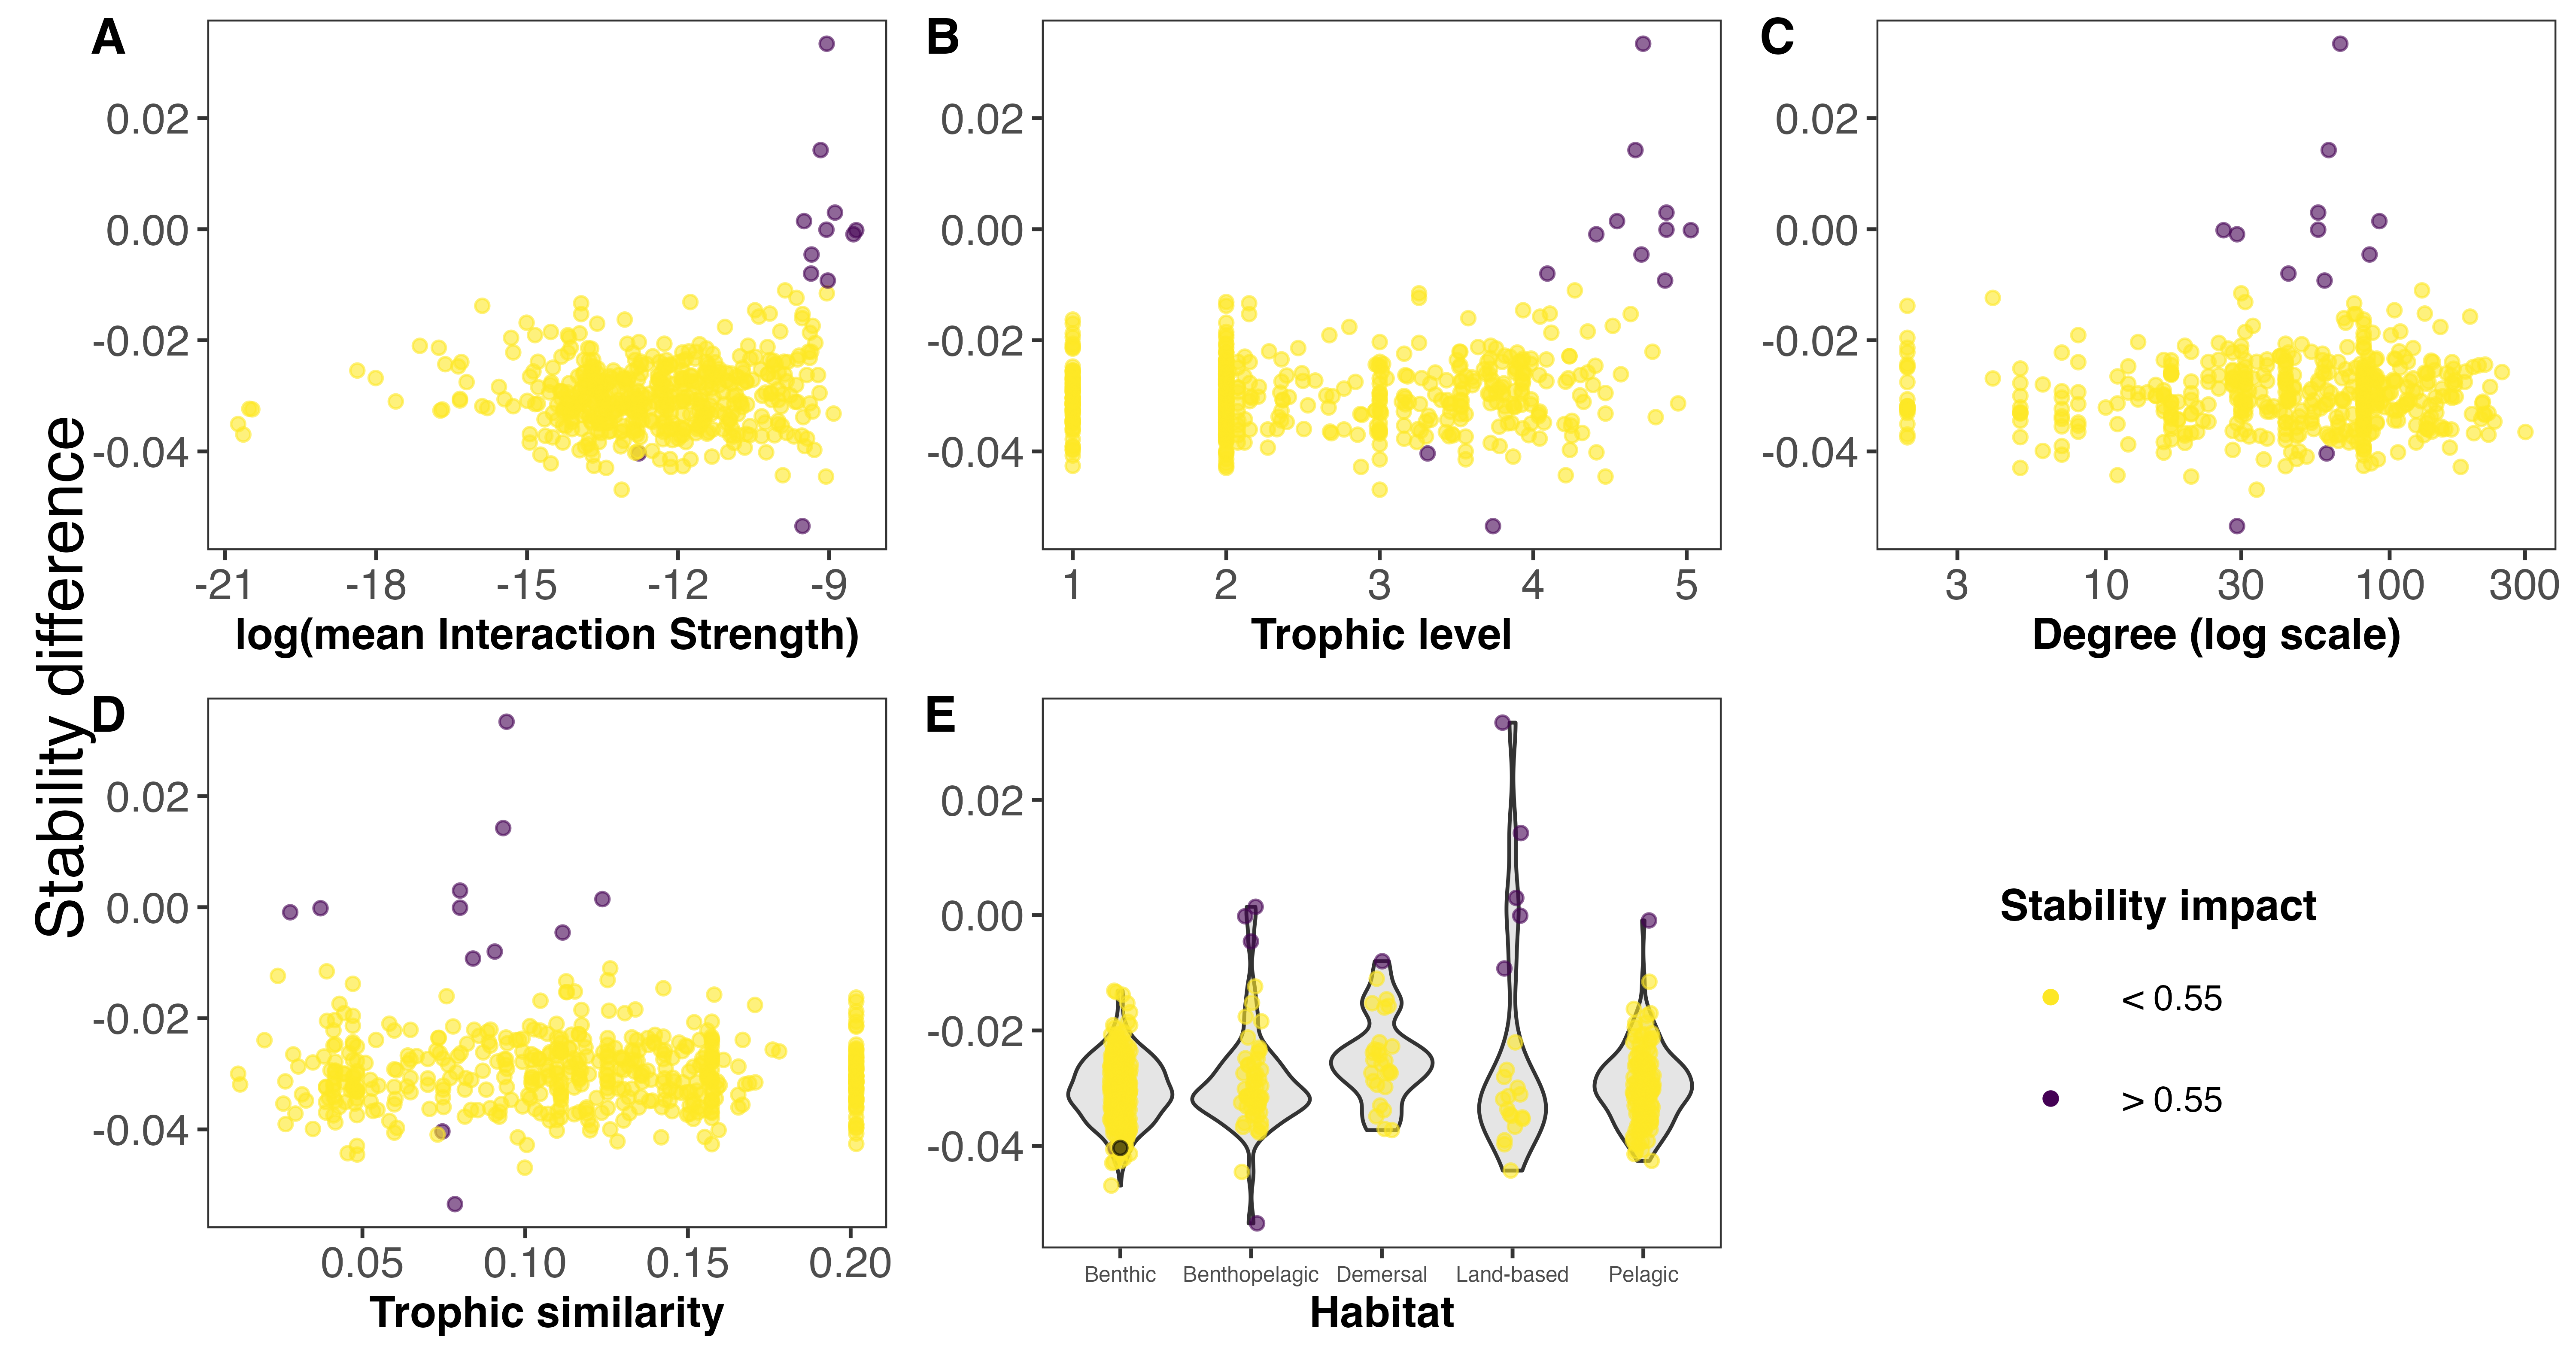
\includegraphics[width=12cm]{Fig.5_QSSDif} \caption{Quasi-Sign Stability (QSS) difference between the whole Weddell Sea food web (n = 490) and the food web without one species (n = 489) for weighted (interaction strength) and unweighted species properties, and habitat. Point color indicates the impact on the QSS; if significant the extinction of that species altered the stability (QSS) of the food web.}\label{fig:unnamed-chunk-5}
\end{figure}

\clearpage

\begin{table}[t]
\caption{Model comparison for the distribution of interaction strengths of the Weddell Sea food web. Order by best fit. References: df = degrees of freedom, AIC = Akaike Information Criterion, deltaAIC = difference with best fit. Log-Normal is the best model.}
\begin{tabular}{l c c c}
\tophline

\textbf{Model} & \textbf{df} & \textbf{AIC} & \textbf{deltaAIC} \\
\middlehline
log-Normal & 2 & -359738 & 0 \\
\middlehline
Gamma & 2 & -359714.1 & 23.89 \\
\middlehline
Power-law & 2 & -350667 & 9070.97 \\
\middlehline
Exponential & 1 & -327606.5 & 32131.54 \\
\middlehline
Normal & 2 & -291407.8 & 68330.21 \\
\middlehline
Uniform & 2 & -248179 & 111559.02 \\

\bottomhline
\end{tabular}
\end{table}

\clearpage

\begin{table}[t]
\caption{Properties of the species that when become extinct generated a significant impact on the stability of the Weddell Sea food web, ordered by significance (Anderson-Darling p-value). References: meanIS = mean interaction strength, TL = trophic level, Deg = degree, TS = trophic similarity, StabDif = stability difference, ADvalue = Anderson-Darling p-value.}
\begin{tabular}{l c c c c c c c}
\tophline

\textbf{Species} & \textbf{meanIS} & \textbf{TL} & \textbf{Deg} & \textbf{TS} & \textbf{Habitat} & \textbf{StabDif} & \textbf{ADvalue}\\
\middlehline
Orcinus orca & 1.83e-4 & 5.03 & 26 & 0.037 & Benthopelagic & 4.67e-5 & 2.28e-41 \\
\middlehline
Macrourus holotrachys & 8.30e-5 & 4.70 & 85 & 0.112 & Benthopelagic & 3.55e-5 & 2.73e-23 \\
\middlehline
Pagetopsis macropterus & 7.08e-5 & 4.64 & 76 & 0.113 & Demersal & -1.80e-5 & 2.38e-12 \\
\middlehline
Abyssorchomene nodimanus & 2.56e-5 & 4.21 & 137 & 0.130 & Benthopelagic & 2.30e-5 & 8.52e-10 \\
\middlehline
Dissostichus mawsoni & 7.82e-5 & 4.12 & 87 & 0.126 & Pelagic & 2.17e-5 & 1.57e-9 \\
\middlehline
Macrourus whitsoni & 7.14e-5 & 4.55 & 92 & 0.124 & Benthopelagic & 2.12e-5 & 3.30e-8 \\
\middlehline
Hydrurga leptonyx & 1.03e-4 & 4.72 & 67 & 0.094 & Land-based & 2.04e-5 & 9.66e-6 \\
\middlehline
Mesonychoteuthis hamiltoni & 1.80e-4 & 4.41 & 29 & 0.028 & Pelagic & 1.82e-5 & 4.59e-5 \\
\middlehline
Champsocephalus gunnari & 7.62e-5 & 3.72 & 46 & 0.086 & Pelagic & 1.83e-5 & 6.79e-5 \\
\middlehline
Notothenia marmorata & 8.27e-5 & 4.09 & 44 & 0.091 & Demersal & 1.60e-5 & 1.23e-4 \\
\middlehline
Arctocephalus gazella & 9.28e-5 & 4.67 & 61 & 0.093 & Land-based & 1.17e-5 & 2.09e-4 \\
\middlehline
Trematomus pennellii & 3.04e-5 & 4.04 & 192 & 0.158 & Demersal & 1.44e-5 & 1.00e-3 \\
\middlehline
Mirounga leonina & 1.20e-4 & 4.87 & 56 & 0.080 & Land-based & 1.41e-5 & 1.28e-3 \\
\middlehline
Notothenia coriiceps & 4.94e-5 & 4.27 & 130 & 0.126 & Demersal & 1.44e-5 & 1.66e-3 \\
\middlehline
Maxilliphimedia longipes & 2.21e-6 & 3.26 & 60 & 0.136 & Benthopelagic & -4.46e-6 & 9.74e-3 \\

\bottomhline
\end{tabular}
\end{table}

\appendixfigures
\clearpage

\begin{figure}
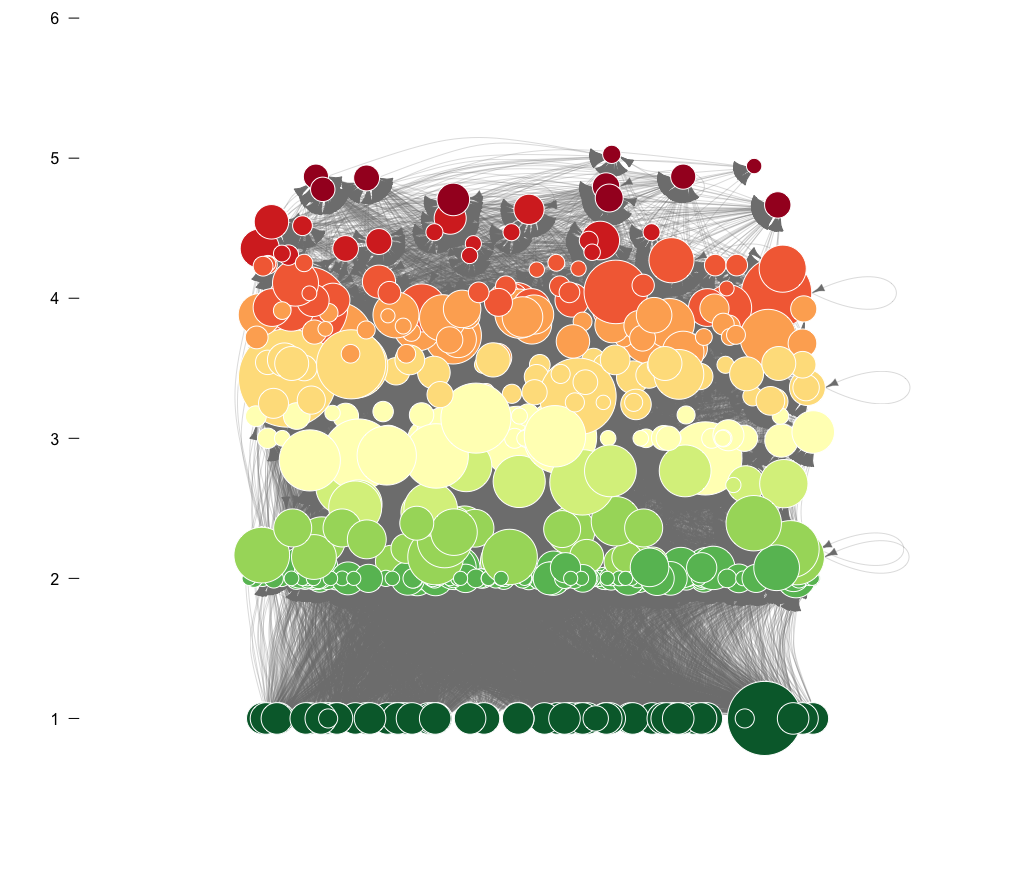
\includegraphics[width=12cm]{App1_FWplot} \caption{Graphic representation of the Weddell Sea food web. Species (nodes) are arranged vertically and colored by trophic level. The diameter of the node indicates the total number of interactions. Predator-prey interactions are represented by the arrows, from prey to predator.}\label{fig:unnamed-chunk-6}
\end{figure}






%%%%%%%%%%%%%%%%%%%%%%%%%%%%%%%%%%%%%%%%%%
%% optional

%%%%%%%%%%%%%%%%%%%%%%%%%%%%%%%%%%%%%%%%%%

%%%%%%%%%%%%%%%%%%%%%%%%%%%%%%%%%%%%%%%%%%
\authorcontribution{TIM and LAS: Conceptualization (lead); Data curation
(lead); Formal analysis (lead); Methodology (lead); Coding (lead);
Writing -- original draft (lead); Writing -- review and editing (lead).
SK: Conceptualization (lead); Formal analysis (supporting); Methodology
(supporting); Coding (supporting); Writing -- original draft
(supporting); Writing -- review and editing
(supporting).} %% optional section

%%%%%%%%%%%%%%%%%%%%%%%%%%%%%%%%%%%%%%%%%%
\competinginterests{The authors declare no competing
interests.} %% this section is mandatory even if you declare that no competing interests are present

%%%%%%%%%%%%%%%%%%%%%%%%%%%%%%%%%%%%%%%%%%

%%%%%%%%%%%%%%%%%%%%%%%%%%%%%%%%%%%%%%%%%%
\begin{acknowledgements}
Thanks to the rticles contributors!
\end{acknowledgements}

%% REFERENCES
%% DN: pre-configured to BibTeX for rticles

%% The reference list is compiled as follows:
%%
%% \begin{thebibliography}{}
%%
%% \bibitem[AUTHOR(YEAR)]{LABEL1}
%% REFERENCE 1
%%
%% \bibitem[AUTHOR(YEAR)]{LABEL2}
%% REFERENCE 2
%%
%% \end{thebibliography}

%% Since the Copernicus LaTeX package includes the BibTeX style file copernicus.bst,
%% authors experienced with BibTeX only have to include the following two lines:
%%
\bibliographystyle{copernicus}
\bibliography{../WeddellSea.bib}
%%
%% URLs and DOIs can be entered in your BibTeX file as:
%%
%% URL = {http://www.xyz.org/~jones/idx_g.htm}
%% DOI = {10.5194/xyz}


%% LITERATURE CITATIONS
%%
%% command                        & example result
%% \citet{jones90}|               & Jones et al. (1990)
%% \citep{jones90}|               & (Jones et al., 1990)
%% \citep{jones90,jones93}|       & (Jones et al., 1990, 1993)
%% \citep[p.~32]{jones90}|        & (Jones et al., 1990, p.~32)
%% \citep[e.g.,][]{jones90}|      & (e.g., Jones et al., 1990)
%% \citep[e.g.,][p.~32]{jones90}| & (e.g., Jones et al., 1990, p.~32)
%% \citeauthor{jones90}|          & Jones et al.
%% \citeyear{jones90}|            & 1990


\end{document}
